\documentclass[10pt,a4paper]{book}
\usepackage[utf8]{inputenc}
\usepackage[T1]{fontenc}
\usepackage{amsmath}
\usepackage{amsthm}
\usepackage{ctex}
\usepackage{amsfonts}
\usepackage{amssymb}
\usepackage{graphicx}

\usepackage{listings}   % include the package before using it

\newtheorem{theorem}{Theorem}[section]
\newtheorem{lemma}{Lemma}[section]
\newtheorem{corollary}{Corollary}[section]

%//LaTeX 头部添加
%\newtheorem{theorem}{Theorem}[section]
%
%\begin{theorem}
%	***//定理内容
%	\label{thm-1}
%\end{theorem}
%
%\begin{proof}
%	***//证明过程
%\end{proof}
%
%//LaTeX 头部添加
%\newtheorem{lemma}{Lemma}[section]
%
%\begin{lemma} 
%	***//引理内容
%	\label{lem-1}
%\end{lemma}
%
%//LaTeX 头部添加
%\newtheorem{corollary}{Corollary}[section]
%
%\begin{corollary} 
%	***//推论内容
%	\label{cor-1}
%\end{corollary}


\usepackage{geometry}
%\geometry{right=2.0cm,left=2.0cm}% 。设置左右两侧页边距都是2厘米
%同时,如果想要设置上下页边距的话:
\geometry{right=2.0cm,left=2.0cm,top = 2.0cm, bottom = 2.0cm}
%奇偶页左右两侧页边距不同

%\geometry{a4paper,scale=0.8}
%————————————————
%版权声明:本文为CSDN博主「nccccc12345」的原创文章,遵循CC 4.0 BY-SA版权协议,转载请附上原文出处链接及本声明。
%原文链接:https://blog.csdn.net/nccccc12345/article/details/115335255

\begin{document}
	\chapter{2020年笔记}
	\section{20.07.27}
	\begin{equation}
		\begin{aligned}
			I &= \int_{\frac{\pi}{4}}^{\pi}\int_{0}^{2\sin\theta} f(r\cos\theta,r\sin\theta)r\text{d}r\text{d}\theta\\	
			&=[\int_{0}^{\sqrt{2}}\int_{\frac{\pi}{4}}^{\pi-\arcsin\frac{r}{2}} 
			+ \int_{\sqrt{2}}^{2} \int_{\arcsin\frac{r}{2}}^{\pi-\arcsin\frac{r}{2}}  ]
			f(r\cos\theta,r\sin\theta)r\text{d}r\text{d}\theta\\
		\end{aligned}
	\end{equation}
	
	\section{20.08.03}
	
	\begin{equation}
		\lim\limits_{n \rightarrow +\infty }
	(1-\frac{1}{1+2})(1-\frac{1}{1+2}) (1-\frac{1}{1+2+3})\dots(1-\frac{1}{1+2+\dots+n}) = ?
	\end{equation}

	\begin{equation}
		\begin{aligned}
			1-\frac{1}{\frac{n(n+1)}{2}} &= 1-\frac{2}{n(n+1)}\\
			&=\frac{n^2+n-2}{n(n+1)}\\
			&=\frac{(n+2)(n-1)}{n(n+1)}
		\end{aligned}
	\end{equation}
	
	\begin{equation}
		\begin{aligned}
			I&=\lim\limits_{n\rightarrow +\infty}\frac{1\times 4}{2\times 3}\frac{2\times 5}{3\times 4}\dots \frac{(n-2)(n+1)}{(n-1)n}\frac{(n-1)(n+2)}{n(n+1)}\\
			&=\lim\limits_{n\rightarrow+\infty}\frac{1}{3}\frac{4}{2}\frac{2}{4}\frac{5}{3}\frac{3}{5}\frac{6}{4}\dots \frac{n+2}{n}\\
			&=\lim\limits_{n\rightarrow+\infty}\frac{1}{3}\frac{n+2}{n}\\
			&=\frac{1}{3}\lim\limits_{n \rightarrow +\infty }\frac{n+2}{n}\\
			&=\frac{1}{3}
		\end{aligned}
	\end{equation}
	\\
	\\
	\\
	卡塔兰数 $ C_n $
	
	从0开始 $ 1, 1, 2, 5, 14, 42, \dots $
	\[
	C_{n+1} = C_0 C_n + C_1 C_{n-1} + \dots + C_n C_0
	\]
	
	该公式的证明可以通过
	\[
	\Bigg( \bigg( \Big( \big( \Bigg) \bigg) \Big) \big)
	\]
	如图所示的括号匹配,$ C_n $可以看成上面四组括号的合理排列形式,(合理排列意味着每一对括号都是左右对应的,像$ )( $这样的形式是非法的)
	
	在$ n $对括号的排列中,假设最后一个括号和第$ i $个左括号匹配。则在第$ i $个左括号之前,一定已经匹配上了$ (i-1) $对左括号。如下图,因此,此种情况的数量为$ f(i-1)*f(n-i-1) $。$ (1\leq i\leq n) $最后一个右括号可以$ 1 \sim n $个左括号匹配共n种情况。
	
	\begin{figure} [h]
		\centering
		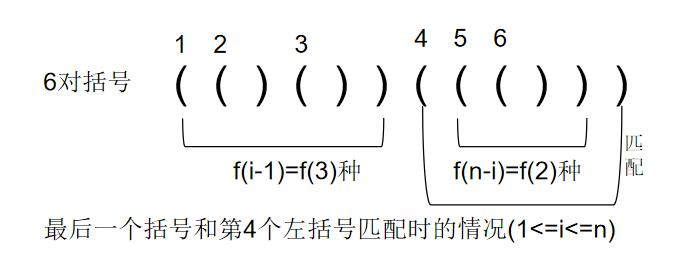
\includegraphics[width=0.7\linewidth]{pic/catalan_proof-001}
		\caption{catalan number - proof}
		\label{fig:catalanproof-001}
	\end{figure}
	
	
%	\[
%???	(n-3)C_n = \frac{n}{2}(C_3 C_{n-1} + C_4 C_{n-2} + \dots + C_{n-2} C_4 + C_{n-1} C_3 )
%	\]
	第$ n+1 $项 
	\[C(n) = \frac{C^n_{2n}}{n+1} \]
	\[	C(n) = C_{2n}^n-C_{2n}^{n-1} = \frac{C_{2n}^n}{n+1}	\]
	
	通项公式
	\[ C_1 = 1, C_n = C_{n-1}\frac{4n-2}{n+1} \]
	
	
	Python 实现
	
	
	\begin{lstlisting}[language=Python]
		# 打印前 n 个卡特兰数
		ans, n = 1, 20
		print("1:" + str(ans))
		for i in range(2, n + 1):
		ans = ans * (4 * i - 2) // (i + 1)
		print(str(i) + ":" + str(ans))
	\end{lstlisting}
	
	
	扩展\\
	
	最后留一道比较有意思的卡特兰数问题,欢迎读者留言,提出自己的看法。
	
	8 个高矮不同的人需要排成两队,每队 4 个人。其中,每排都是从低到高排列,且第二排的第 i 个人比第一排中第 i 个人高,则有多少种排队方式。
	
	
	
	\section{20.08.07}
	
	\begin{theorem}
	A-G 不等式\\ 任意n个非负实数$ a_1, a_2, \dots, a_n$ \\
	\begin{equation}
		\frac{a_1 + a_2 + \dots + a_n}{n} \geq \sqrt[n]{a_1\dots a_n}
	\end{equation}
	其中等号成立 $\iff a_1 = a_2 = \dots = a_n$

	\label{thm-1}
	\end{theorem}

	\begin{proof}\label{1}
	数学归纳法\\ $n=1$时结论平凡\\
	$n=2\qquad \frac{a_1+a_2}{2} \geq \sqrt{a_1a_2}$\\
	\[(a_1 - a_2)^2 = a_1^2 - 2 a_1 a_2 + a_2^2 \geq 0 \]
	\[a_1^2 + 2a_1a_2 + a_2^2 \geq 4a_1a_2\]
	\[(a_1+a_2)^2\geq 4a_1a_2\]
	\[\frac{a_1+a_2}{2}\geq \sqrt{a_1a_2}\]
	$n=k$时,假设 $\frac{a_1+\dots+a_k}{k}\geq \sqrt[k]{a_1\dots a_k}$成立\\
	$ n=k+1 $
	\begin{equation}
	\begin{aligned}
		&\frac{a_1+\dots + a_k + a_{k+1}}{k+1}-\frac{a_1+\dots +a_k}{k} \\
		=&\frac{k(a_1+\dots+a_{k+1})-(k+1)(a_1+\dots+a_k)}{k(k+1)}\\
		=&\frac{ka_{k+1}-(a_1+\dots+a_k)}{k(k+1)}\\		
	\end{aligned}
	\end{equation}
	we found 
	\[\frac{a_1+\dots + a_k + a_{k+1}}{k+1} =  \frac{a_1+\dots + a_k}{k} + \frac{ka_{k+1}-(a_1+\dots + a_k)}{k(k+1)} \]
	note \[ A := \frac{a_1+\dots + a_k}{k} , \qquad B:=\frac{ka_{k+1}-(a_1+\dots + a_k)}{k(k+1)}\]
	
	\begin{equation}
		(\frac{a_1+\dots + a_k + a_{k+1}}{k+1})^{k+1}=(A+B)^{k+1}\geq A^{k+1}+(k+1)A^k B
	\end{equation}
	使用二项式展开需要对$ a_i $从小到大重排,而使用Bernoulli不等式则只需要$ A\geq 0, (A+B)\geq 0 $即可
	\begin{equation}
		A^{k+1}+(k+1)A^k B = A^k(A+(k+1)B)
	\end{equation}
	\begin{equation}
		\begin{aligned}
			A^k& =	(\frac{a_1+\dots + a_k + a_{k+1}}{k+1})^{k+1} \geq a_1\dots a_k \quad \text{assume at}(n=k)\\
			A+(k+1)B&= \frac{a_1+\dots + a_k}{k} + \frac{ka_{k+1}-(a_1+\dots + a_k)}{k} = a_{k+1}\\
			\because& (A+B)^{k+1}\geq A^k(A+(k+1)B)\geq a_1 \dots a_k  a_{k+1}\\
			\therefore & 	\frac{a_1+\dots + a_k + a_{k+1}}{k+1} \geq  \sqrt[k+1]{a_1 \dots a_k  a_{k+1}}\\
		\end{aligned}
	\end{equation}
	
	使用二项式展开定理的条件:\\
	在归纳法第二步对$a_1 \dots a_{k+1}  $重编号,使$ a_{k+1} $为其中最大的数(之一)\\
	这使得分解式右边第二项$ \frac{ka_{k+1}-(a_1+\dots+a_k)}{k(k+1)} $ 一定是非负数
	\end{proof}
	
	
	\begin{proof}\label{证明 2}
	Forward and backward (Cauchy, 1897)\\
	Forward Part:\\
	$ n=2 $ 
	\begin{equation}
		\frac{a_1+a_2}{2}\geq \sqrt{a_1a_2}
	\end{equation}
	$ n=4 $ 
	\begin{equation}
		\begin{aligned}
			\frac{a_1+a_2+a_3+a_4}{4}
			&\geq \sqrt{\frac{a_1+a_2}{2}\frac{a_3+a_4}{2}}\\
			&\geq \sqrt{\sqrt{a_1a_2}\sqrt{a_3a_4}}\\
			&\geq \sqrt[4]{a_1a_2a_3a_4}\\
		\end{aligned}
	\end{equation}
	$ n=2^k $ 假设不等式$ \frac{a_1+\dots +a_{2^k}}{2^k}\geq \sqrt[2^k]{a_1\dots a_{2^k}} $成立\\
	$ n=2^{k+1} $
	\begin{equation}
		\begin{aligned}
			\frac{a_1+\dots+a_{2^k}+\dots+a_{2^{k+1}}}{2^{k+1}}
			&\geq \sqrt{\frac{a_1+\dots +a_{2^k}}{2^k}\frac{a_{2^k+1}+\dots +a_{2^{k+1}}}{2^k}}\\
			&\geq \sqrt{\sqrt[2^k]{a_1\dots a_{2^k}}\sqrt[2^k]{a_{2^k+1}\dots a_{2^{k+1}}}}\\
			&\geq \sqrt[2^{k+1}]{a_1\dots a_{2^{k+1}}}
		\end{aligned}
	\end{equation}
	
	Backward Part:
	A-G不等式对某个$ n\geq 2 $成立,则它对$ n-1 $也成立
	\begin{equation}
		\begin{aligned}
			\frac{1}{n-1}\sum_{i=1}^{n-1}a_i 
			&= \frac{1}{n}(\frac{n}{n-1})\sum_{i=1}^{n-1}a_i\\
			&=\frac{1}{n}(\sum_{i=1}^{n-1}a_i+\frac{1}{n-1}\sum_{i=1}^{n-1}a_i)
		\end{aligned}
	\end{equation}
	将$ \frac{1}{n-1}\sum_{i=1}^{n-1}a_i $看作$ a_n $
	\begin{equation}
		\frac{1}{n-1}\sum_{i=1}^{n-1}a_i
		\geq \sqrt[n]{(\prod_{i=1}^{n-1}a_i) (\frac{1}{n-1}\sum_{i=1}^{n-1}a_i)}
	\end{equation}
	
	\begin{equation}	
		(\frac{1}{n-1}\sum_{i=1}^{n-1}a_i)^n
		\geq \prod_{i=1}^{n-1}a_i(\frac{1}{n-1}\sum_{i=1}^{n-1}a_i)
	\end{equation}
	

	\begin{equation}	
		(\frac{1}{n-1}\sum_{i=1}^{n-1}a_i)^{n-1}
		\geq \prod_{i=1}^{n-1}a_i
	\end{equation}


	\begin{equation}		
		\frac{1}{n-1}\sum_{i=1}^{n-1}a_i
		\geq \sqrt[n-1]{\prod_{i=1}^{n-1}a_i}
	\end{equation}


	\begin{equation}
		\frac{1}{n-1}\sum_{i=1}^{n-1}a_i \geq \sqrt[n]{(\prod_{i=1}^{n-1}a_i)(\frac{1}{n-1}\sum_{i=1}^{n-1}a_i)}
	\end{equation}
	
	\begin{equation}
		( \frac{1}{n-1}\sum_{i=1}^{n-1}a_i )^n \geq \prod_{i=1}^{n-1}a_i(\frac{1}{n-1}\sum_{i=1}^{n-1}a_i)
	\end{equation}

	\begin{equation}
		( \frac{1}{n-1}\sum_{i=1}^{n-1}a_i )^{n-1} \geq \prod_{i=1}^{n-1}a_i
	\end{equation}
	
	\begin{equation}
		 \frac{1}{n-1}\sum_{i=1}^{n-1}a_i  \geq \sqrt[n-1]{\prod_{i=1}^{n-1}a_i}
	\end{equation}
	
	\end{proof}
	
	\begin{theorem}
		柯西,施瓦茨不等式\\	
		对$ a_1,\dots,a_n $和$ b_1, \dots ,b_n \in \mathbb{R}$,成立
		\begin{equation}
			|\sum_{i=1}^n a_ib_i|\leq \sqrt{\sum_{i=1}^n a_i^2}\sqrt{\sum_{i=1}^n b_i^2}
		\end{equation}
		\label{1.3.5}
	\end{theorem}
	\begin{proof}
		\[ \sum_{i=1}^n (a_i - \lambda b_i)^2 = \sum_{i=1}^n a_i^2 - 2\lambda \sum_{i=1}^n a_i b_i + \lambda^2 \sum_{i=1}^n b_i^2 \geq 0  \]
		由韦达定理(视$ \lambda $为未知数),原方程无解或只有唯一解
		
		\begin{equation}
			\begin{aligned}
				 \Delta = b^2-4ac \leq 0\\
				 (-2\sum_{i=1}^n a_i b_i)^2-4\sum_{i=1}^na_i^2\sum_{i=1}^nb_i^2\leq 0\\	
				 (\sum_{i=1}^n a_i b_i)^2 \leq \sum_{i=1}^na_i^2\sum_{i=1}^nb_i^2\\
				 \sum_{i=1}^n a_i b_i \leq \sqrt{\sum_{i=1}^na_i^2}\sqrt{\sum_{i=1}^nb_i^2}\\
			 \end{aligned}
		\end{equation}
	\end{proof}

	\section{20.08.11}
\begin{theorem}	定积分第一中值定理\\
	设函数$ f(x),g(x) \in \mathbb{C}[a,b]. $且在$ [a,b] $上不变号,则存在$ \zeta \in  [a,b]$,使得$ \int_{a}^{b}f(x)g(x) = f(\zeta)\int_{a}^bg(x)\text{d}x $
	
\end{theorem}
\begin{proof}
	suppose that $ g(x)\ge 0 $. $ f(x) $ continuous on close set,so we can get the maximum and minimum value of $ f $. We note that m is the minimum value of $f(x), x\in [a,b] $,and M is the maximum value of $ f(x) $, then we have:

	\begin{gather}
		mg(x) \le f(x)g(x) \le Mg(x)\\
		m\int_{a}^{b}g(x)\text{d}x \le \int_{a}^{b}f(x)g(x)\text{d}x\le M\int_{a}^{b}g(x)\text{d}x
	\end{gather}

	note that we don't know$ \int_{a}^{b}g(x)\text{d}x \neq 0$
	
	When $ \int_{a}^{b}g(x)\text{d}x = 0$, then $ g(x) \equiv 0 $, So $ \forall \zeta \in [a,b] $, the theorem works.
	
	When $ \int_{a}^{b}g(x)\text{d}x = 0$, then $ m\le \frac{\int_{a}^{b}f(x)g(x)\text{d}x}{\int_{a}^{b}g(x)\text{d}x} \leq M $
	
	From the Intermediate Value Theorem, $ f(x) \in \mathbb{C}[a, b] \quad m\le f(x) \le M $
	
	\begin{gather}
		\exists \zeta \in [a,b] \quad f(\zeta) = \frac{\int_{a}^{b}f(x)g(x)\text{d}x}{\int_{a}^{b}f(x)\text{d}x}\\
		\int_{a}^{b}f(x)g(x)\text{d}x = f(\zeta)\int_{a}^{b}g(x)\text{d}x
	\end{gather}

\end{proof}

设$ g(x) $在$ [a,b] $上连续可积,$ f(x) $在$ [a,b] $上连续单调递增,且$ f'(x) \ge 0 $,并对$ \forall x\in [a,b] $ 有$ f(x)\ge 0 $。则存在$ \zeta \in [a,b] $,使得
\begin{gather}
	\int_{a}^{b}f(x)g(x)\text{d}x = f(b)\int_{\zeta}^{b}g(x)\text{d}x
\end{gather}

\begin{proof}
	set$ G(x) = \int_{x}^{b}g(t)\text{d}t , g(x)\text{在}[a,b] $	上可积

	则$ G(x),x\in [a,b] $存在最值,设最小值和最大值分别为$ m,M $
	
	\begin{gather}
		G(x) = -\int_{b}^{x}g(t)\text{d}t,\quad  G'(x) = -g(x)
	\end{gather}

\begin{equation}
	\begin{aligned}
		\int_{a}^{b}f(x)g(x)\text{d}x &= -\int_{a}^{b}f(x)\text{d}G(x)\\
		&=-{(f(b)G(b) - f(a)G(a)) -\int_{a}^{b}G(x)f'(x)\text{d}x }\\
		&= f(a)G(a)+ \int_{a}^{b}G(x)f'(x)\text{d}x\\
	\end{aligned}
\end{equation}
	\begin{gather}
		m\int_{a}^{b}f'(x)\text{d}x \le \int_{a}^{b} G(x)f'(x)\text{d}x \le M\int_{a}^{b}f'(x)\text{d}x\\
		m[f(b-f(a))] \le  \int_{a}^{b} G(x)f'(x)\text{d}x \le M[f(b-f(a))]\\
	\end{gather}
$ \because $
	\begin{gather}
		mf(a) \le  f(a)G(a) \le Mf(a)\\	
		mf(b) \le  \int_{a}^{b} f(x)g(x) \text{d}x \le Mf(b)\\	
	\end{gather}
\begin{equation}
	\begin{gather}
		\text{when} f(b)=0,    &f(x)\equiv 0, \forall \zeta \in [a,b], \text{等式恒成立}\\
		\text{when} f(b)\neq0, &m\le \frac{\int_{a}^{b}f(x)g(x)\text{d}x}{f(b)}\le M\\
	\end{gather}
\end{equation}
	From the Intermediate Value Theorem, $ \exists \zeta \in [a,b] s.t. G(\zeta) = \frac{\int_{a}^{b}f(x)g(x)\text{d}x}{f(b)} $\\
	then we have
	\begin{gather}
		\int_{a}^{b}f(x)g(x)\text{d}x = f(b)G(\zeta) = f(b)\int_{\zeta}^{b}g(x)\text{d}x
	\end{gather}
	
	
\end{proof}



	\section{20.08.12}
	1.3.2 练习题
	
	1. 关于Bernoulli不等式的推广:
	\\(1) 证明:当$ -2\ge h\ge -1 $时Bernoulli不等式$ (1+h)^n \ge 1+nh $仍成立;\\
	(2) 证明:当$ h\ge 0 $时成立不等式 
	\begin{equation}
		(1+h)^n\ge \frac{n(n-1)h^2}{2}
	\end{equation} 
	(3) 证明:若$ a_i>-1 \quad (i=1,2,\dots,n) $且同号,则成立不等式\\
	solve:\\
	(1)
	\[ -2 \leq h \leq -1 \]
	\[ -1 \leq 1+h \leq 0 \]
	\[ -1 \leq (1+h)^n \leq 0 \]
	\[ -2n \leq nh \leq -n \]
	\[ 1-2n \leq 1+nh \leq 1-n \]
	
	$ n=0 \qquad (1+h)^0 = 1 = 1+0*h $  结果是平凡的
	
	$ n=1 \qquad 1+h = 1+h $ 结果是平凡的
	
	$ n \geq 2 \qquad $ 此时 $ 1-n \leq -2 $
	\[ 0 \geq (1+h)^n \geq -1 \geq -2 \geq 1-n \geq 1-nh \geq 1- 2n  \]
	\[ (1+h)^n \geq 1+nh \]
	\\
	(2) 
	\[ h\geq 0 \qquad (1+h)^n \geq \frac{n(n-1)h^2}{2} \]
	\[ (1+h)^n=1+nh+\frac{n(n-1)}{2}h^2 + \dots \geq \frac{n(n-1)}{2}h^2  \]
	
	推广:
	\[ (1+h)^n \geq C_n^3 h^3, C_n^4 h^4, \dots , C_n^k h^k ,\qquad 0\leq k\leq n\]
	\\
	(3) 
	\[ \prod_{i=1}^n (1+a_i)\ge 1+\sum_{i=1}^n a_i \]
	(a)$ a_i \ge 0$, 且同号。 
	\[ \prod_{i=1}^n (1+a_i) = 1+ \sum_{i=1}^n a_i + \sum_{i=1,i\neq j}^n \sum_{j=1}^n a_i a_j + \sum_{i=1,i\neq j,k}^n \sum_{j=1,j\neq k}^n \sum_{k=1}^n a_i a_j a_k+\dots \]
	\[ \prod_{i=1}^n (1+a_i) \geq \frac{\prod_{i=1}^n(1+a_i)}{1+a_k} \qquad \forall k\in 1,2,\dots , n,\quad 1+a_k \geq 1 \]
	\\
	(b) $ 0 > a_i > -1 \text{此时} 1 > 1+a_i > 0$
%	\[ \prod_{i=1}^n(1+a_i) \in (0, 1) \]
%	\[ 0> \sum_{i=1}^n a_i >-n \qquad 1>1+\sum_{i=1}^n  a_i >1-n\]
%	\[\text{记}b_i := 1+a_i\qquad a_i = b_i -1, 0<b_i<1\]
%	\[ \prod_{i=1}^n(1+a_i) = \prod_{i=1}^nb_i \]
%	\[1+\sum_{i=1}^na_i = 1+\sum_{i=1}^n(b_i-1)=\sum_{i=1}^n b_i-(n-1)\]
%	$ b_i \in(0,1) $,由A-G不等式
%	\[\frac{1}{n}\sum_{i=1}^n b_i \ge \sqrt[n]{\prod_{i=1}^n b_i}\]
%	\[ \frac{1}{2n-1}[\sum_{i=1}^n b_i - (n-1)] \ge \sqrt[2n-1]{\prod_{i=1}^n b_i\cdot 1^{n-1}} \]
%	\[ \frac{1}{2n-1}[\sum_{i=1}^n a_i + 1] \ge \sqrt[2n-1]{\prod_{i=1}^n (a_i + 1)\cdot 1^{n-1}} \]
	\\别人的方法:
	$ n=1 $时不等式变成等式,显然成立\\
	设$ n=k $时不等式也成立
	\[ \prod_{i=1}^k(1+a_i)\ge 1+\sum_{i=1}^k a_i\]
	则$ n=k+1 $时,有
	\[ \prod_{i=1}^{k+1}(1+a_i) = \prod_{i=1}^k a_i (1 + a_{k+1}) \ge (1+\sum_{i=1}^k a_i) (1+a_{k+1})\]
	\[(1+\sum_{i=1}^k a_i) (1+a_{k+1})=1+\sum_{i=1}^k a_i + a_{k+1} + \sum_{i=1}^k a_i\cdot a_{k+1} \ge 1+\sum_{i=1}^{k+1} a_i \]
	\[\therefore \prod_{i=1}^{k+1}(1+a_i)\ge 1+\sum_{i=1}^{k+1} a_i\]
	
	
	2. 利用A-G不等式求解下列有关阶乘$ n! $的不等式\\
	(1)证明:当$ n>1 $时成立
	\begin{equation}
		n!<(\frac{n+1}{2})^n 
	\end{equation}
	(2)利用$ (n!)^2 = (n\cdot 1)((n-1)\cdot 2)\dots(1\cdot n) $证明:当$ n>1 $时成立
	\begin{equation}
		n!<(\frac{n+2}{\sqrt{6}})^n
	\end{equation}
	(3)比较(1)(2)两个不等式的优劣,并说明原因;\\
	(4)证明:对任意实数$ r $成立
	\begin{equation}
		(\sum_{k=1}^n k^r)^n \ge n^n(n!)^r
	\end{equation}
	solve:\\
	(1) when $ n>1 $
	\[  n! = 1\times 2\times\dots\times n < (\frac{1+2+\dots + n}{n})^n  \]
	\[ (\frac{1+2+\dots + n}{n})^n = (\frac{n(n+1)}{2n})^n = (\frac{n+1}{2})^n \]
	(2) when $ n>1 $
	\[ (n!)^2 = (n\cdot 1)((n-1)\cdot 2)\dots(1\cdot n) < (\frac{n\cdot 1 + (n-1)\cdot 2 + \dots + 1\cdot n}{n})^n \]
	\begin{equation}
		\begin{aligned}
			n\cdot 1 + (n-1)\cdot 2 + \dots + 1\cdot n &= \sum_{k=1}^n (n-k+1)k \\
			\sum_{k=1}^n (n-k+1)k 
			&= (n+1)\sum_{k=1}^n k-\sum_{k=1}^n k^2\\
			&= (n+1)\frac{n(n+1)}{2}-\frac{n(2n+1)(n+1)}{6}\\
			&= \frac{n(n+1)}{6}(3(n+1)-(2n+1))\\
			&= \frac{n(n+1)(n+2)}{6}
		\end{aligned}
	\end{equation}
	
	\begin{equation}
		\begin{aligned}
			(n!)^2  &= (n\cdot 1)((n-1)\cdot 2)\dots(1\cdot n)\\
					&< (\frac{n\cdot 1 + (n-1)\cdot 2 + \dots + 1\cdot n}{n})^n\\
					&= (\frac{1}{n}\frac{n(n+1)(n+2)}{6})^n\\
					&= (\frac{(n+1)(n+2)}{6})^n\\
					&< (\frac{n+2}{6})^{2n}
		\end{aligned}
	\end{equation}

	\begin{equation}
		\therefore \qquad	n! < (\frac{n+2}{\sqrt{6}})^{n}
	\end{equation}
	
	(3) 
	\begin{equation}
		\frac{n+1}{2} = \frac{n+2}{\sqrt{6}}
	\end{equation}
	解得$ n=1+\sqrt{6} >3 $, 
	$ n>3 $时 (2)式更精确,结果比(1)式更好。
	
	(4) $ \forall r \in \mathbb{R} \quad (n!)^r \le \frac{1}{n^n}(\sum_{k=1}^n k^r)^n$
	由A-G不等式
	\begin{equation}
		\frac{1}{n}\sum_{k=1}^n k^r \ge \sqrt[n]{\prod_{k=1}^n k^r}
	\end{equation}
	\begin{equation}
		\begin{aligned}
			(n!)^r  = \prod_{k=1}^n k^r\le (\frac{1}{n}\sum_{k=1}^n k^r)^n =\frac{1}{n^n}(\sum_{k=1}^n k^r)^n
		\end{aligned}
	\end{equation}
	
	\section{20.08.13}
	2.(4) 
	\begin{equation}
		\begin{aligned}
			\forall r \in \mathbb{R} \qquad (\sum_{i=1}^n k^r)^n \ge n^n(n!)^r \\
			 (n!)^r = \prod_{k=1}^n k^r \le (\frac{1^r+2^r+\dots + n^r}{n})^n = \frac{1}{n^n}(\sum_{k=1}^n k^r)^n \quad \text{A-G inequality} \\
			 \therefore (\sum_{k=1}^n k^r)^n \ge n^n(n!)^r\\
		\end{aligned}
	\end{equation}
	
	3. $ a_k >0, \quad k=1,2,\dots, n $ 证明几何-调和平均值不等式
	\begin{equation}
		(\prod_{k=1}^n a_k)^{\frac{1}{n}}\ge \frac{n}{\sum_{k=1}^n\frac{1}{a_k}}
	\end{equation}	
	\begin{proof}
		from A-G inequality 
		\begin{equation}
			\begin{aligned}
				\frac{\sum_{k=1}^n\frac{1}{a_k}}{n} &\ge \sqrt[n]{\prod_{k=1}^n \frac{1}{a_k}} \\
				& =  \frac{1}{\sqrt[n]{\prod_{k=1}^n{a_k}}}\\
				\therefore a_k>0, \qquad {\sqrt[n]{\prod_{k=1}^n{a_k}}}&\ge \frac{n}{\sum_{k=1}^n\frac{1}{a_k}}
			\end{aligned}
		\end{equation}
		
	\end{proof}
	
	
	4. $ a,b,c \ge 0 $, proof that
	\begin{equation}
		\sqrt[3]{abc}\le \sqrt{\frac{ab+bc+ca}{3}}\le\frac{a+b+c}{3}
	\end{equation}
	并推广到n个非负数的情况
	\begin{proof}
		\text{left:}\\
		\begin{equation}
			\begin{aligned}
				\sqrt[3]{abc} &=\sqrt{\sqrt[3]{ab\cdot bc\cdot ca}}\\
				&\le \sqrt{\frac{ab+bc+ca}{3}}
			\end{aligned}
		\end{equation}
		\text{right:}
		\begin{equation}
			\begin{aligned}
				\sqrt{\frac{ab+bc+ca}{3}} &\le \sqrt{\frac{
						(\frac{a+b}{2})^2+
						(\frac{b+c}{2})^2+
						(\frac{c+a}{2})^2
					}{3}}\\
				&=\sqrt{\frac{2(a^2+b^2+c^2)+2(ab+bc+ca)}{12}}\\
				&=\sqrt{\frac{a^2+b^2+c^2+ab+bc+ca}{6}}\\				
			\end{aligned}
		\end{equation}
	
	\begin{equation}
		\because a,b,c \ge 0 \qquad 	\frac{ab+bc+ca}{3} \le \frac{a^2+b^2+c^2+ab+bc+ca}{6}
	\end{equation}
	需要证明 $ \sqrt{\frac{ab+bc+ca}{3}}\le\frac{a+b+c}{3} $\\
	对该式两边平方
	\begin{equation}
		{\frac{ab+bc+ca}{3}}\le\frac{(a+b+c)^2}{9} = \frac{a^2+b^2+c^2 + 2ab+2bc+2ca}{9}
	\end{equation}
	
	\begin{equation}
		\begin{aligned}
			\frac{ab+bc+ca}{3}  &\le \frac{a^2+b^2+c^2}{6} + \frac{ab+bc+ca}{6}\\
								&\le \frac{a^2+b^2+c^2}{6} + \frac{ab+bc+ca}{3}\\
								&= (\frac{a+b+c}{3})^2 \\
			\therefore 	\sqrt{\frac{ab+bc+ca}{3}}  &\le  \frac{a+b+c}{3}\\
		\end{aligned}
	\end{equation}

	\end{proof}
	
	\begin{proof}
		\text{推广至n个}
		\begin{equation}
			\begin{aligned}[l]
				n=2\qquad & \sqrt{ab}      &\le& \frac{a+b}{2} & & \\
				n=3\qquad & \sqrt[3]{abc}  &\le& \sqrt{\frac{ab+bc+ca}{3}}   &\le& \frac{a+b+c}{3}\\
%				n=4\qquad & \sqrt[4]{abcd} &\le \sqrt[3]{\frac{abc+bcd+cda+dab}{4}}    
%				&\le \sqrt{\frac{ab+bc+cd+da}{4}}  &\le \frac{a+b+c+d}{4}  \\
				n=k\qquad & \sqrt[k]{\prod_{i=1}^k a_i}       &\le& \sqrt{\frac{\sum_{i=1}^k-1a_ia_{i+1} + a_ka_1}{k}} &\le& \frac{\sum_{i=1}^ka_i}{k} &\\
			\end{aligned}
		\end{equation}
		
		\begin{equation}
			\text{1} \qquad
			\sqrt[k]{a_1a_2\dots a_k} = \sqrt{\sqrt[k]{a_1^2a_2^2\dots a_k^2}}\le\sqrt{\frac{a_1a_2+a_2a_3+\dots a_ka_1}{k}}
		\end{equation}
		
		\begin{equation}
			\text{2} \qquad
			\sqrt{\frac{a_1a_2+a_2a_3+\dots a_ka_1}{k}} \le \frac{a_1+\dots + a_k}{k}
		\end{equation}
		
		\begin{equation}
			\begin{aligned}
				\frac{a_1a_2+a_2a_3+\dots a_ka_1}{k} &\le \frac{a_1^2 + \dots a_k^2}{2k}\\
				2\frac{a_1a_2+a_2a_3+\dots a_ka_1}{k} &\le \frac{(a_1 + \dots a_k)^2}{2k}\\
				\sqrt{\frac{a_1\dots a_k}{k}} &\le \frac{a_1+\dots +a_k}{\sqrt{4k}}\quad\text{wrong!}
			\end{aligned}
		\end{equation}
		
		
		
	\end{proof}
	
\end{document}